\chapter{Alternative Termination Conditions} \label{sec:alttercdns}
 This chapter explores some of the possible Collatz Variants. Before we investigate them, we define a graph paradigm that transforms the $3N+1$ problem into directed graphs that depict the flow for all input numbers modulo base $b$, where $b$ is a power of 2. Using this paradigm, we can show that some variants are easily provable. However, others are not.
\section{Base \textit{b} Collatz Graph Definition} \label{subsec:colgraph}
Define $G_b=(V,E)$ to be a ``Base $b$ Collatz Graph'', where $b = 2^k$, and $k$ is nonnegative. Choosing a power of 2 for $b$ allows us to easily reason with binary numbers, which is useful for both several proofs in this chapter and the Collatz SRS that we will discuss starting in Chapter~\ref{sec:SRSandSAT}. \hl{$V$ has $b$ vertices in it, where each vertex is labeled a unique integer in the interval $[0, b-1]$. We say that a number $N$ is visiting vertex $v \in V$ if and only if $N \equiv v \Mod{b}$ for vertex $v$ labelled with integer $v$. Out of convenience, note that we use $v$ as a vertex and integer interchangeably in this paper. %\par

%, when we refer to vertex $v$, we are referring both to the vertex $v \in V$, and a number $v$, such that $N$ visiting the vertex labelled $v$ means $N \equiv v \Mod{b}$.

% We often use the vertex label $v$ and numbers interchangeably, so if we say ``node $v$'', we are talking about $v \Mod{b}$ and the vertex $v \in V$ interchangeably. This is done out of conveneince.
%This thesis uses the term ``node $v$'' as shorthand to correspond to the number $v$ in $v \Mod{b}$, as opposed to ``vertex $v$'' which corresponds to the actual vertex of the graph. 

Let $N$ be an input number, and $N_1$ the result of applying the $3N+1$ mapping to $N$. $E = V \times V$ is a set of directed edges, where, for nodes $u, v \in V$, $(u,v) \in E$ if and only if $N_i \equiv u \Mod{b}$ and $N_{i+1} \equiv v \Mod{b}$ for some $N$ and $N_1$.}

\section{Base \textit{b} Collatz Graph Lemmas}
This section contains some lemmas that are used throughout this chapter. First, we start with a lemma about the number of node transitions in any Collatz Base $b$ Graph $G_b$.
\begin{lemma}
\label{lem:numOutEdges}
Given a Collatz Base $b$ Graph, for all $v \in V$, if node $v$ is even, then it has two outgoing edges. Otherwise, if node $v$ is odd, then it has only one outgoing edge.
\end{lemma}
\begin{proof}
\hl{Take some number $N$ that is visiting node $v$, and consider $N$ in binary. First, let us consider the case where node $v$ is even. When we divide by 2, we just remove the lowest 0 bit from $N$ to get $N_{1}$. The bit at index $k-1$ of $N_{1}$ can be either a 0 or a 1, allowing for two options for even nodes. \par
Now, let $N$ visit an odd node $v$. Multiplying $N$ by 3 and adding 1 will give us a $N_1$ where the binary string for it grows at least one bit longer than $N$, since $3\cdot N = 2 \cdot N + N$, and $2N$ in binary is shifting the bits of $N$ one index to the left, then adding a 0 bit to the least significant bit. This gives us only one option for the least significant $k$ bits, meaning $N_1$ can only visit one node, and only one such outgoing edge from $v$ exists.}
\end{proof}
Now, we have a couple of important properties about cycles that exist in any Collatz Base $b$ Graph, and the fact that these cycles cannot continue indefinitely. First, we introduce the ``0 cycle'' lemma.
\begin{lemma}
\label{lem:zeroCycle}
For any Collatz Base $b$ Graph (where $b$ is a positive power of 2), a self-loop occurs on a 0 node. This cycle cannot continue indefinitely.
\end{lemma}
\begin{proof}
Assume we have an input number $N$ such that $N \equiv 0 \Mod{b}$. This means that the $k$ least significant bits are all 0. Apply the $3N+1$ mapping once to this string. We remove a 0 from the end, since we divide the input number by 2. We now look at the new number $N_1$ and the $k$ least significant bits. The $k-1$ least significant bits are all 0. But what is the value of the bit in the most significant of the $k$ lowest bits of $N_1$? If it is a 0, then $N_1 \equiv 0 \Mod{b}$, and we have a self-loop. \par
To show that the self loop cannot continue indefinitely: every time we follow the self-loop, remove a 0. Since we also know that $N > 1$ in order for the algorithm to continue running, we also know that at least one binary digit is a 1. So as we continue dividing by 2 and removing bits that are 0, we eventually reach, after $i$ visits to node 0, a point where the least $k$ significant bits are $1000\ldots 0$, meaning $N_i$ is visiting node $b/2$ instead, ending the cycle.
\end{proof}
Now, we introduce another important lemma about cycles: the fact that we will always have a cycle between nodes $b-2$ and $b-1$, and it cannot continue indefinitely.
\begin{lemma}
\label{lem:oneConsumption}
 For any Collatz Base $b$ Graph, a cycle between exists between nodes $b-2$ and $b-1$. This cycle cannot continue indefinitely.
\end{lemma}
\begin{proof}
In this proof, we will show first that a $b-1 \rightarrow b-2 \rightarrow b-1$ cycle exists, and second, that this cycle cannot continue indefinitely; more precisely, that some number congruent modulo to $b-2 \Mod{b}$, after division by 2, actually becomes congruent modulo to $b/2-1 \Mod{b}$ instead. We will prove this using long multiplication in binary. \par
%x NEEDS to remain x here, make it equal to some number N
Let $x$ be a arbitrary number\footnote{\hl{Normally, we use the notation $N$ to denote an arbitrary number in the $3N+1$ sequence, but we mean $N_i$ to mean the $i$\textsuperscript{th} number in the $3N+1$ sequence, whereas in this proof, we have $x_j$ to denote the $j$\textsuperscript{th} bit of $x$. Hence, we use variables $x$ and $y$ instead of $N$ and $N_1$.}} congruent modulo to $b-1 \Mod{b}$. We want to express $x$ in binary, so let $x$ have $m$ bits. We know that since $x$ is congruent modulo to $b-1 \Mod{b}$, all bits from indices 0 to $k-1$ are 1. Let $x_j$ denote the $j$\textsuperscript{th} bit of $x$, $k \leq j \leq m$. These bits are unknown. Let $1_{+1}$ correspond to the adding of 1 after multiplying by 3, which is added to the least significant bit of $x$. Let $c_j$ denote the unknown carry for the $j$\textsuperscript{th} addition of bits. Let $y$ be the result after $3x+1$ is computed, and let index $j$ of $y$ be the same index as $x$. The multiplication is referenced in Figure~\ref{fig:mul}. \par
\begin{figure}
\begin{tabular}{*{16}c}%{c*{15}{@{\,}c}}
 & & $ x_{n}$  & $ x_{n-1}$  & \ldots & $ x_{j+1}$  & $ x_{j}$  & \ldots & $ x_{k+1}$  & $ x_{k}$  & 1 & 1 & \ldots & 1 & 1 & 1 \\
$\times$ & & & & & & & & & & & & & & 1 & 1 \\
\hline
\tiny ${\scriptscriptstyle c_{n+2}}$ & ${\scriptscriptstyle c_{n+1}}$ & ${\scriptscriptstyle c_{n}}$ & ${\scriptscriptstyle c_{n-1}}$ & & ${\scriptscriptstyle c_{j+1}}$ & ${\scriptscriptstyle c_{j}}$ & & ${\scriptscriptstyle c_{k+1}}$ & \tiny 1 & \tiny 1 &  \tiny 1 & &  \tiny 1 & \tiny 1 & \\
  & & $ x_{n}$  & $ x_{n-1}$  & \ldots & $ x_{j+1}$  & $ x_{j}$  & \ldots & $ x_{k+1}$  & $ x_{k}$  & 1 & 1 & \ldots & 1 & 1 & 1 \\
  + & $ x_{n}$  & $ x_{n-1}$  & $ x_{n-2}$  & \ldots & $ x_{j}$  & $ x_{j-1}$  & \ldots & $ x_{k}$  & 1 & 1 & 1 & \ldots & 1 & 1 & $1_{+1}$  \\
  \hline
  $ y_{n+2}$  & $ y_{n+1}$  & $ y_{n}$  & $ y_{n-1}$  & \ldots & $ y_{j+1}$  & $ y_{j}$  & \ldots & $ y_{k+1}$  & $ y_{k}$  & 1 & 1 & \ldots & 1 & 1 & 0 
\end{tabular}
\caption{The long multiplication corresponding to $3x + 1$. Note how, in the addition step, the $1_{+1}$ is in place of a zero, and the addition is just $x + 2x + 1$.}
\label{fig:mul}
\end{figure}
As mentioned in lemma~\ref{lem:numOutEdges}, multiplication of a binary number $x$ by 3 is just $x + 2x$, and $2x$ is just placing all bits of $x$ one index to the left, adding a 0 bit at the newly vacant spot. In the multiplication we show in Figure~\ref{fig:mul}, we write this but replace the new least signifcant 0 bit of $2x$ with the special $1_{+1}$ bit, allowing us to perform $3x+1$ with just one addition instead of two. \par
Notice that all bits in the resulting binary number $y$ from indices 0 to $k-1$ are 1, except for index 0, which is 0. This is because all bits of $y$, save the least significant bit, are computed by adding $1+1$ and carrying over the 1 from the previous addition. As a result, $y$ is congruent modulo to $b-2 \Mod{b}$, meaning an edge from node $b-1 \Mod{b}$ to node $b-2 \Mod{b}$ exists in our graph.\par
When we divide $y$ by 2, we just remove the least significant 0 bit from $y$, decreasing the indices of all bits in $y$ by 1. Hence, bit $y_k$ is now in position $k-1$. If $y_k$ is 1, our number is now congruent modulo to $b-1 \Mod{b}$. This means an edge also exists from node $b-2 \Mod{b}$ to node $b-1 \Mod{b}$, proving the existence of the $b-2 \rightarrow b-1 \rightarrow b-2$ cycle. \par
Now we show that this cycle will always eventually terminate. This happens when, after dividing a number congruent modulo to $b-2 \Mod{b}$ by 2, bit $y_{k-1}$ is 0. So we need to show this eventually occurs for any positive integer $x$. There are two cases for this:
\begin{enumerate}
    \item Some bit in $x$ is 0. Let $x_j$ be the least significant bit of $x$ that is 0 (all bits which have indices lower than $j$ are 1). Look back at Figure~\ref{fig:mul}, and replace $x_j = 0$, and have all bits at indices less than $j$ be 1. After taking the $3x+1$ step, all bits of $y$ between 1 and $j-1$ will be 1, since for each bit, we add $1 + 1$ and carry over a 1. However, when we get to index $j$, we add $1 + 0$ plus a carry of 1, making bit $y_j = 0$. Since after we divide by 2 we move all bits one index to the right, bit $y_j$ now moves to index $j-1$. We repeat this process a total of $j-k+1$ times. After this, the 0 bit will be in position $y_{k-1}$, making $y$ congruent modulo to $b/2 - 1 \Mod{b}$ instead, breaking the cycle.
    \item No bit in $x$ is 0. In this case, again looking at Figure~\ref{fig:mul}, all bits in $y$ from indices 1 to $m$ will be 1. However, bit $y_{m+1} = 0$, because $y_{m+1} = c_{m+1} + x_{m} + x_{m+1}$, and $c_{m+1} = 1$ and $x_{m} = 1$, but $x_{m+1} = 0$. Since bit $y_{m+1} = 0$ we move it over one index to index $m$ after dividing by 2. We then follow case 1, where $j = m$, and hence, the cycle also breaks in this case.
 \end{enumerate}
 Hence, no input number can follow the $b-2 \rightarrow b-1 \rightarrow b-2$ cycle indefinitely. 
\end{proof}
We introduce one more lemma that shows that cycles where the magnitude of divisions by 2 outweigh the magnitude of multiplications by 3. We call this the ``even node dominance lemma''.
\begin{lemma}
\label{lem:EvenDom}
Given a cycle in any Collatz Base $b$ Graph $G$, let $V_{e}$ be the set of even nodes in the cycle, and $V_{o}$ be the set of odd nodes. If $2^{|V_e|} > 3^{|V_o|}$, then the cycle cannot continue indefinitely.
\end{lemma}
\begin{proof}
Let $2^{|V_e|} > 3^{|V_o|}$ \hl{and $j=|V_e| + |V_o|$. Let $N$ be visiting a node $v$ in the cycle, and assume $N$ will run through the cycle at least once without terminating, implying no number between $N$ and $N_j$ inclusive is 1, and that $N_j$ visits the same node $v$ as $N$ did.} We visited $|V_e|$ vertices in the cycle, so we divided $N$ by $2^{|V_e|}$ after one trip around the cycle. We also visited $|V_o|$ vertices in the cycle, each time multiplying by 3, and overall, multiplied $N$ by about $3^{|V_o|}$.\footnote{We also added one each time we visit an odd node, but this is asymptotically insignificant compared to multiplying by 3 or dividing by 2, so we ignore it in this proof.}\par
Hence, after we visited the cycle once, we computed $N_{j} \approx \frac{3^{|V_o|}}{2^{|V_e|}}N$. Since $2^{|V_e|} > 3^{|V_o|}$, $N_{j} < N$. Therefore, one of two things must happen:
\begin{enumerate}
\item $N$ eventually becomes 1, which means the cycle no longer can be repeated.
\item The cycle is eventually broken.
\end{enumerate}
In both cases, the cycle cannot continue indefinitely.
\end{proof}
\section{Base 4 Collatz Graph and Variants} \label{subsec:base4graph}
\hl{In this section, we build a simple example of a Base $b$ Collatz Graph:  $G_4$. We chose $G_4$ because we can prove that $\ColMod{N}{A}{4}$ terminates for any nonempty $A \subseteq \{0,1,2,3\}$. In $G_4$, there are 4 different nodes: one for each integer between 0 and 3. When determining which node $v$ input number $N$ visits, we look at the lowest 2 bits of $N$, since $4= 2^2$. For example, $N \equiv 0\Mod{4}$ has 00 as the 2 least significant bits, whereas $N \equiv 2\Mod{4}$ has 10 as its 2 least significant bits.}
 \subsection{Base 4 Collatz Graph Construction} \label{subsubsec:proofbase4graph}
Figure~\ref{fig:base_4_graph} shows \hl{$G_4$. We describe the construction in this subsection. We start by describing the transitions for even nodes, then the transitions for odd nodes. Assume, in all cases, that a number $N$ is written in binary. First, the transitions for even nodes:}
\begin{figure}
    \centering
    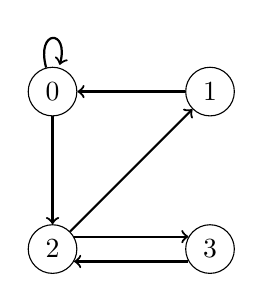
\begin{tikzpicture}
    \node[shape=circle,draw=black] (A) at (0,2) {0};
    \node[shape=circle,draw=black] (B) at (2,2) {1};
    \node[shape=circle,draw=black] (C) at (0,0) {2};
    \node[shape=circle,draw=black] (D) at (2,0) {3};
    \path  (A) edge [loop above, thick] (A);
    \path [->] (B) edge [thick] (A);  
    \path [->] (A) edge [thick] (C);  
    \path [->] (C) edge [thick] (B);  
    \path [->] (C.30) edge [thick] (D.150);  
    \path [->] (D.210) edge [thick] (C.-30);  
    \end{tikzpicture}
    \caption{The Base 4 Collatz Graph, $G_4$. There are 4 nodes, each one corresponding to a value mod 4.}
    \label{fig:base_4_graph}
\end{figure}

\begin{itemize}
    \item \hl{$N$ visiting node 0 means $N$ ends with binary string ``00''. Removing the last 0 bit of $N$ leaves either ``00'', meaning $N_1$ visits node 0 again, or ``10'', meaning $N_1$ visits node 2 instead.} 
    \item \hl{$N$ visiting node 2 means $N$ ends with binary string ``10''. Removing the last 0 bit of $N$ leaves either ``01'', meaning $N_1$ visits node 1, or ``11'', meaning $N_1$ visits node 3.}
\end{itemize}
Now, the transitions for odd nodes. Let $x_2$ and $x_3$ be unknown bits:
\begin{itemize}
    \item \hl{$N$ visiting node 1 means $N$ ends with binary string ``01''.  Multiplying this by 3 and adding 1 results in $N_1$ ending with ``$x_200$'', so $N_1$ visits node 0.}
    \item \hl{$N$ visiting node 3 means $N$ ends with binary string ``11''.  Multiplying this by 3 and adding 1 results in $N_1$ ending with ``$x_3x_210$'', so $N_1$ visits node 2.}
\end{itemize}
\subsection{Base 4 Collatz Variants} \label{subsubsec:base4variants}
We introduced the Base 4 case for nodes because we can prove that we need to visit all of the nodes in this graph, which is equivalent to saying that each of the Collatz Variants, $\ColMod{N}{A}{4}$ terminates for nonempty $A \subseteq \{0,1,2,3\}$, and for any input number $N$. 
\begin{theorem}
$\ColMod{N}{A}{4}$ terminates for nonempty $A \subseteq \{0,1,2,3\}$.
\end{theorem}
\begin{proof}
\hl{Assume that no $3N+1$ sequence described in this proof reaches 1, otherwise $\ColMod{N}{A}{4}$ terminates trivially for any $A$.} We will start with proving that $\ColMod{N}{\{2\}}{4}$ will terminate for any input number $N$, because the 2 node is central to the Base 4 graph.  \par
\begin{lemma}
\label{lem:collatzSubTwoModFour}
$\ColMod{N}{\{2\}}{4}$ terminates for any $N$.
\end{lemma} 
\begin{proof}
We use the graph to help in this proof. An equivalent question is this: Can we show that node 2 must be visited for all input numbers? To show that this is the case, we have to show that all other nodes must visit node 2.
\begin{itemize}
    \item 2: \hl{If the input number $N$ is visiting node 2, we are already done.}
    \item 3: \hl{If the input number $N$ is visiting node 3, then after the $3N+1$ mapping is applied to $N$, $N_1$ is now visiting node 2.}
    \item 1 and 0: \hl{Let $N$ be visiting node 1. $N_1$ visits node 0 after applying the $3N+1$ mapping once. To show $N_{1+j}$ must leave node 0}, we use lemma~\ref{lem:zeroCycle} (the ``0 cycle'' lemma) for $b = 4$, \hl{and $N_{1+j}$ will visit node 2 after $j$ more applications of the $3N+1$ mapping, both causing $\ColMod{N}{\{2\}}{4}$ to terminate.}
\end{itemize}
Since all other nodes must visit node 2, it means that for all $N$, $\ColMod{N}{\{2\}}{4}$ terminates.
\end{proof} \par

\begin{lemma}
\label{lem:collatzSubOneModFour}
$\ColMod{N}{\{1\}}{4}$ terminates for any $N$.
\end{lemma}
\begin{proof}
We use lemma~\ref{lem:collatzSubTwoModFour} \hl{to show that node 2 must be visited, meaning that for any input number $N$, $N_i \equiv 2 \Mod{4}$ after $i$ steps. Then we use lemma}~\ref{lem:oneConsumption} \hl{to show that the cycle between nodes 2 and 3 cannot continue indefinitely, so after $j$ more steps, $N_{i+j}$ visits node 1, proving termination of this variant.}
\end{proof}
\begin{lemma}
\label{lem:collatzSubZeroModFour}
$\ColMod{N}{\{0\}}{4}$ terminates for any $N$.
\end{lemma}
\begin{proof}
Given lemma~\ref{lem:collatzSubOneModFour}, we know after $i$ steps $N_i$ must visit node 1, and given lemma~\ref{lem:numOutEdges}, an odd node can only have one outgoing edge, so $N_{i+1}$ visits node 0.
\end{proof}
\begin{lemma}
\label{lem:collatzSubThreeModFour}
$\ColMod{N}{\{3\}}{4}$ terminates for any $N$.
\end{lemma}
\begin{proof}
Given the ``even node dominance lemma'',~\ref{lem:EvenDom}, \hl{the $2 \rightarrow 1 \rightarrow 0 \rightarrow \ldots \rightarrow 2$ cycle cannot continue forever because, if we assume that the 0 node never self-cycles, $2^2 > 3^1$. The 0 self-cycle makes even nodes dominate even more. So an input number $N$ in the $2 \rightarrow 1 \rightarrow 0 \rightarrow \ldots \rightarrow 2$ cycle must, after $i$ steps, visit node 3, causing $\ColMod{N}{\{3\}}{4}$ to terminate.}
\end{proof}
Since all of these lemmas hold, it follows that any singleton set from $A \subseteq \{0,1,2,3\}$ causes $\ColMod{N}{A}{4}$ to terminate. Also, by definition of Algorithm~\ref{alg:ColSP}, any larger size sets for $A$ also terminate as larger set sizes add more termination conditions. So any nonempty set $A$ will cause $\ColMod{N}{A}{4}$ to terminate for any input $N$.
\end{proof}
\section{Base 8 Collatz Graph and Variants} \label{subsec:base8graphsubpblms}
After proving $\ColMod{N}{A}{4}$ terminates for any nonempty base set $A$ and input number $N$, we decided to see what would happen if we expanded to $k = 3$ bits. We have not been able to prove all variants of $\ColMod{N}{A}{8}$ for all nonempty sets $A$. This will motivate further computation undertaken in Chapter~\ref{sec:subhrdnspred}, as we try to determine how hard figuring out these unproven variants are. Figure~\ref{fig:base_8_graph} shows the base 8 graph. There are 8 different nodes, since $8 = 2^3$.
\begin{figure}
    \centering
    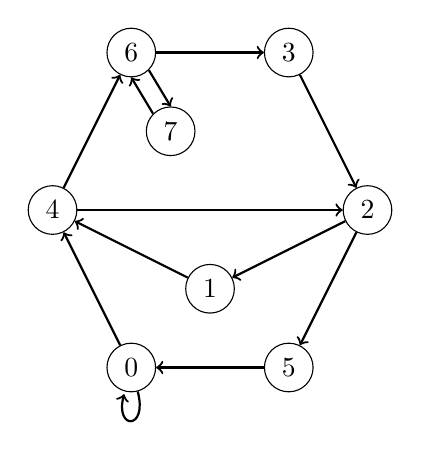
\begin{tikzpicture}
    \node[shape=circle,draw=black] (A) at (1,0) {0};
    \node[shape=circle,draw=black] (B) at (2,1) {1};
    \node[shape=circle,draw=black] (C) at (4,2) {2};
    \node[shape=circle,draw=black] (D) at (3,4) {3};
    \node[shape=circle,draw=black] (E) at (0,2) {4};
    \node[shape=circle,draw=black] (F) at (3,0) {5};
    \node[shape=circle,draw=black] (G) at (1,4) {6};
    \node[shape=circle,draw=black] (H) at (1.5,3) {7};
    \path  (A) edge [loop below, thick] (A);
    \path [->] (A) edge [thick] (E);  
    \path [->] (B) edge [thick] (E);  
    \path [->] (C) edge [thick] (B);  
    \path [->] (C) edge [thick] (F);  
    \path [->] (D) edge [thick] (C);  
    \path [->] (E) edge [thick] (C);  
    \path [->] (E) edge [thick] (G);  
    \path [->] (F) edge [thick] (A);  
    \path [->] (G) edge [thick] (D);  
    \path [->] (G.-45) edge [thick] (H.90);  
    \path [->] (H.135) edge [thick] (G.-90);  
    \end{tikzpicture}
    \caption{The Base 8 Collatz Graph, $G_8$. There are 8 nodes, each one corresponding to a value mod 8.}
    \label{fig:base_8_graph}
\end{figure}

\subsection{Base 8 Collatz Graph Construction} \label{subsubsec:base8proof}
Like $G_4$ before, we show how to construct $G_8$. We examine the even nodes first. In this case, there are four different nodes: 0, 2, 4, and 6. Using lemma~\ref{lem:numOutEdges}, each vertex has two different transitions, depending on what the next bit to the left of the 3 bits after removing the least significant 0. % \item \hl{$N$ visiting node 2 means $N$ ends with binary string ``10''. Removing the last 0 bit of $N$ leaves either ``01'', meaning $N_1$ visits node 1, or ``11'', meaning $N_1$ visits node 3.}


\begin{itemize}
    \item $N$ visiting node 0 means $N$ ends with binary string ``000''. Removing the last 0 bit of $N$ leaves either ``000'', meaning $N_1$ loops to node 0; or ``100'', meaning $N_1$ visits node 4 instead.
    \item $N$ visiting node 2 means $N$ ends with binary string ``010''. Removing the last 0 bit leaves either ``001'', meaning $N_1$ visits node 1; or ``101'', meaning $N_1$ visits node 5.
    \item $N$ visiting node 4  means $N$ ends with binary string ``100''. Removing the last 0 bit leaves either ``010'', meaning $N_1$ visits node 2; or ``110'', meaning $N_1$ visits node 6.
    \item $N$ visiting node 6 means $N$ ends with binary string ``110''. Removing the last 0 bit leaves either ``011'',  meaning $N_1$ visits node 3, or ``111'',  meaning $N_1$ visits node 7.
\end{itemize}
Now, the odd nodes. Let $x_3$ and $x_4$ be unknown bits.
%    \item \hl{$N$ visiting node 1 means $N$ ends with binary string ``01''.  Multiplying this by 3 and adding 1 results in $N_1$ ending with ``$x_200$'', so $N_1$ visits node 0.}
\begin{itemize}
    \item $N$ visiting node 1 means $N$ ends with binary string ``001''. Multiplying this by 3 and adding 1 results in $N_1$ ending with ``$100$'', so $N_1$ visits node 4.
    \item $N$ visiting node 3 means $N$ ends with binary string ``011''. Multiplying this by 3 and adding 1 results in $N_1$ ending with ``$x_3010$'',  so $N_1$ visits node 2.
    \item $N$ visiting node 5 means $N$ ends with binary string ``101''. Multiplying this by 3 and adding 1 results in $N_1$ ending with ``$x_4x_3000$'', so $N_1$ visits node 0.
    \item $N$ visiting node 7 means $N$ ends with binary string ``111''. Multiplying this by 3 and adding 1 results in $N_1$ ending with ``$x_4x_3110$'', so $N_1$ visits node 6.
\end{itemize}
\subsection{Base 8 Collatz Graph Cycle Analysis} \label{subsubsec:cycleanalysis}
Since we do not have proofs for all Collatz Variants $\ColMod{N}{A}{8}$, we analyzed whether certain cycles can last indefinitely. \hl{We have found that all simple cycles of $G_8$ can be proven to not last indefinitely. However, showing that some combinations of these simple cycles cannot continue forever is much more difficult to do.}\par
\hl{We tie in interesting Collatz Variants to these analyses. We start with smaller cycles and work our way into longer cycles, as well as combinations of them.}
\begin{itemize}
    \item The 0 self-cycle, ($0  \rightarrow \ldots$) cannot continue forever, as per lemma~\ref{lem:zeroCycle}.
    \item The $6 \rightarrow 7 \rightarrow 6$ cycle cannot continue forever as per lemma~\ref{lem:oneConsumption}.
    \item The $4 \rightarrow 2 \rightarrow 1 \rightarrow 4$ cycle cannot continue forever, as even nodes dominate ($2^2 > 3$), so according to lemma~\ref{lem:EvenDom}, this cycle cannot last forever.
    \item $4 \rightarrow 2 \rightarrow 5 \rightarrow 0  \rightarrow \ldots \rightarrow 4$ cycle:  Even nodes dominate, even without any 0 self-cycles ($2^3 > 3$), so according to lemma~\ref{lem:EvenDom}, this cycle cannot continue forever. \hl{We can also combine this cycle with the $4 \rightarrow 2 \rightarrow 1 \rightarrow 4$ cycle, and since both cycles cause input numbers to decrease, the combination of these two cycles must visit a new node to prevent the number from converging to 1. The only other choice is node 6, so this argument is used to prove Collatz Variant 6 must terminate.}
    \item $4 \rightarrow 6 \rightarrow 3 \rightarrow 2 \rightarrow 1 \rightarrow 4$ cycle: There are three different variations of this cycle. We have a proof for only one of them:
\begin{itemize}
  \item No transition allowed from $4 \rightarrow 2$: The following theorem explains this case.
  \begin{theorem} Aaronson '17: The $4 \rightarrow 6 \rightarrow 3 \rightarrow 2 \rightarrow 1 \rightarrow 4$ cycle cannot continue indefinitely.
  \end{theorem}
  \begin{proof}
    If we start some number $N$ such that $N \equiv 4\Mod{8}$, and follow the $4 \rightarrow 6 \rightarrow 3 \rightarrow 2 \rightarrow 1 \rightarrow 4$ cycle once, we turn $N$ into $(9N+20)/8 = \frac{9}{8}(N+20)-20$. If we were to repeat the cycle $k$ times, we would turn $N$ into $\frac{9}{8}^k(N+20)-20$. This quantity must be an integer for all $k$ if the cycle is to continue forever. However, $N+20$ will only have a finite number of factors of 8, so the cycle must terminate.
  \end{proof}
  \item Transition allowed between $4 \rightarrow 2$: This creates a conflict between two different cycles: one that causes growth by approximately a factor of $9/8$ ($4 \rightarrow 6 \rightarrow 3 \rightarrow 2 \rightarrow 1 \rightarrow 4$), and another that causes the cycle to decay by a factor of $4/3$ ($4 \rightarrow 2 \rightarrow 1 \rightarrow 4$). Even though we can prove that both of these cycles terminate independently, it has been a challenge to show that the combination of them cannot continue indefinitely, as we cannot prove that one cycle must stop transitioning to the other. Hence, no proof, by hand or machine, is known that we must break out of this combination of cycles, by visiting either node 5 or 7. A proof that this combination of cycles must be broken would prove termination of Collatz Variant $\{5,7\}$, which we explore in Chapter~\ref{sec:subhrdnspred}.
  \item Building on the prior point, we can also consider visits to the node 7 as well in this cycle. This adds the $6 \rightarrow 7 \rightarrow 6$ cycle to the already challenging two cycle case. If we can't prove that the smaller combination of cycles $4 \rightarrow 6 \rightarrow 3 \rightarrow 2 \rightarrow 1 \rightarrow 4$ and $4 \rightarrow 2 \rightarrow 1 \rightarrow 4$ cannot terminate, it would be far more difficult to add a third cycle, even though all three cycles must terminate individually. A proof of this cycle would solve Collatz Variant 5, also explored in Chapter~\ref{sec:subhrdnspred}.
\end{itemize}
\item $4 \rightarrow 6 \rightarrow 3 \rightarrow 2 \rightarrow 5 \rightarrow 0 \rightarrow \ldots \rightarrow 4$ cycle: There are three different variations to showing this cycle cannot continue forever: keeping both nodes 1 and 7 omitted, or omitting one node or the other. Adding in both nodes yields the entire base 8 graph. The variant where both 1 and 7 are omitted is proven, the other two are not.
    \begin{itemize}
        \item Strictly following this cycle, no changes: assuming no zero-cycles, there are 4 distinct even nodes in this cycle, and 2 distinct odd nodes. $2^4 > 3^2$, so according to the ``even node dominiance lemma'',~\ref{lem:EvenDom}, this cycle cannot continue forever. The nodes that must be visited to break this cycle are either 1 or 7, so this is a proof that Collatz Variant $\{1,7\}$ terminates.
        \item Allowing 7 but avoiding 1: Like variant $\{5,7\}$, we have two conflicting cycles: the $6 \rightarrow 7 \rightarrow 6$ cycle which cause the number to grow by approximately $\frac{3}{2}$ every time it takes this cycle, and the base cycle $4 \rightarrow 6 \rightarrow 3 \rightarrow 2 \rightarrow 5 \rightarrow 0 \rightarrow \ldots \rightarrow 4$ that reduces it by approximately $\frac{16}{9}$, depending on number of zero self cycles. These two cycles are interesting in that they clash the fastest growing part of the graph: the $6 \rightarrow 7 \rightarrow 6$ cycle, and the fastest decaying part of the graph: the 0 self-cycle, followed by two more even numbers. We are also not aware of a proof for this case either. Such a proof that these two cycles cannot continue combined forever would be equivalent to proving terminaton of Collatz Variant 1. We present analysis of hardness of this cycle in Chapter~\ref{sec:subhrdnspred}.
        \item Allowing 1 but avoiding 7: Adding back in node 1 but disallowing node 7 actually allows for three different cycles: $4 \rightarrow 6 \rightarrow 3 \rightarrow 2 \rightarrow 5 \rightarrow 0 \rightarrow \ldots \rightarrow 4$, $4 \rightarrow 6 \rightarrow 3 \rightarrow 2 \rightarrow 1 \rightarrow 4$, and $4 \rightarrow 2 \rightarrow 1 \rightarrow 4$.  Finding a proof for this case is expected to be harder than the unsolved two cycle case of $4 \rightarrow 6 \rightarrow 3 \rightarrow 2 \rightarrow 1 \rightarrow 4$, and $4 \rightarrow 2 \rightarrow 1 \rightarrow 4$. Solving that the combination of these three cycles must terminate is equivalent to proving termination of Collatz Variant 7.
    \end{itemize}
\end{itemize}
\subsection{Base 8 Collatz Variants} \label{subsubsec:base8subprob}
As for which nodes we are forced to visit during the computation of a $3N+1$ sequence, we can prove Collatz Variants 2, 3, 4 and 6 terminate, meaning nodes 2, 3, 4, and 6 must be visited in the base 8 graph eventually. Variant 0 can be shown to terminate if another unproven variant terminates. It will still be mentioned with the already proven variants. The following will explain how these five variants terminate. We present them in an order to build arguments off of one another. \hl{Like the proofs for Base 4 Collatz Variants, assume that no $3N+1$ sequence described in this proof reaches 1, otherwise $\ColMod{N}{A}{8}$ terminates trivially for any $A$.}
\begin{itemize}
    \item \textbf{$\boldsymbol{\ColMod{N}{\{6\}}{8}}$:} \hl{Like in the Collatz Base 4 Graph, we have to show that all other nodes must visit node 6 eventually. There are several different cases we enumerate here:}
\begin{enumerate}
\item $N$ visits node 6. We are already done.
\item $N$ visits node 7. Then after one application of the $3N+1$ mapping, $N_1$ visits node 6.
\item $N$ is visiting nodes 0, 1, 2, 4, or 5. The $3N+1$ sequence for $N$ in this case, to avoid node 6, would have to traverse one of two cycles: $4 \rightarrow 2 \rightarrow 1 \rightarrow 4$ or $4 \rightarrow 2 \rightarrow 5 \rightarrow 0 \rightarrow \ldots \rightarrow 4$.  We talked about how this combination of cycles cannot continue forever in Subsection~\ref{subsubsec:cycleanalysis}. So an $N$ input number in either one of these cycles, after $i$ steps, must visit node 6.
\item $N$ visits node 3. Then after one application of the $3N+1$ mapping, $N_1$ visits node 2, and we apply the previous argument to show it must transition to node 6 eventually.
\end{enumerate}  
Hence, $\ColMod{N}{\{6\}}{8}$ must terminate for any input $N$.
    \item \textbf{$\boldsymbol{\ColMod{N}{\{3\}}{8}}$:} We know that $\ColMod{N}{\{6\}}{8}$ terminates, so as a result, an input number $N$ must transition to node 6 after $i$ steps. Given lemma~\ref{lem:oneConsumption}, the $6 \rightarrow 7 \rightarrow 6$ cycle cannot continue forever. Hence, after another $j$ steps, $N_{i+j}$ visits node 3, meaning $\ColMod{N}{\{3\}}{8}$ must terminate.
    \item \textbf{$\boldsymbol{\ColMod{N}{\{2\}}{8}}$:} Since we know that $N$ must visit node 3 after $i$ steps, we apply the $3N+1$ mapping once, and $N_{i+1}$ visits node 2, proving $\ColMod{N}{\{2\}}{8}$ must terminate.
    \item \textbf{$\boldsymbol{\ColMod{N}{\{4\}}{8}}$:} Given that we know we need to visit node 2, we know that $N_i$ visits node 2. We look at the graph and see two different paths, both which lead to node 4: Either visit node 1 then 4, or visit node 5 then 0. From lemma~\ref{lem:zeroCycle}, the 0 cycle cannot continue forever, so either way, the path taken must traverse to node 4. Hence after $j$ steps for $j \geq 2$, $N_{i+j}$ visits node 4, and $\ColMod{N}{\{4\}}{8}$ terminates.
    \item \textbf{$\boldsymbol{\ColMod{N}{\{0\}}{8}}$:} In the graph, we can see that to visit node 0, we must come from node 5. So we cannot prove this yet unless we prove termination for $\ColMod{N}{\{5\}}{8}$.
\end{itemize}
We do not have proofs for $\ColMod{N}{\{1\}}{8}$, $\ColMod{N}{\{5\}}{8}$, $\ColMod{N}{\{7\}}{8}$, but we can prove a couple of combined variants of them:
\begin{itemize}
    \item \textbf{$\boldsymbol{\ColMod{N}{\{1,5\}}{8}}$:} We already know that Collatz Variant 2, so $N_i$ visits node 2. Looking at the base 8 graph, 2 must traverse to either node 1 or 5. Hence, after one application of the $3N+1$ mapping, $N_{i+1}$ visits either 1 or 5, meaning $\ColMod{N}{\{1,5\}}{8}$ must terminate.
    \item \textbf{$\boldsymbol{\ColMod{N}{\{1,7\}}{8}}$:} This was discussed in Subsection~\ref{subsubsec:cycleanalysis}, but repeated here: Since the $4 \rightarrow 6 \rightarrow 3 \rightarrow 2 \rightarrow 5 \rightarrow 0 \rightarrow \ldots \rightarrow 4$ cannot continue forever, either node 1 or 7 must be visited, since there are not other choices for nodes. Hence, $\ColMod{N}{\{1,7\}}{8}$ must terminate.
\end{itemize}
However, the combination $\ColMod{N}{\{5,7\}}{8}$ has not been proven. Hence, we've run some computational experiments to try and better understand the difficulty of coming up with a proof for termination of variant $\{5,7\}$, as well as Collatz Variants 1, 5, and 7.
